\chapter{Database}

Database and database manage systems (DBMS) are introduced in this chapter. Both relational and non-relational databases are covered. Tools and languages to manipulate databases, such as structured query language (SQL) for relational databases, are introduced.

\section{Brief Introduction}

Database, in a broad view, refers to an organized collection of data of any format. In this sense, any file format that hosts information in an meaningful and explainable way, such as \textit{CSV}, \textit{XML} and \textit{JSON}, is a database. These file formats often work fine when the data is stored in a centralized manner and its size small.

As the data size grows, the robustness and efficiency of storing and retrieving data may become an issue, and different database models have been proposed for improved performance. Dedicated software, namely DBMS, are developed to manage and maintain the database and provide an interface for the users to create, retrieve, update and delete data. Different database models require different database engines and DBMS, and different DBMS may provide different interfaces for the users.

There are hundreds of database models available in the market. In general, the most widely seen database models can be divided into two categories, namely the relational databases (RDB) and the non-relational databases.

\subsection{Relational Database}

Relational database was proposed in 1970s by IBM. Some important features of a relational database includes the following.
\begin{itemize}
	\item Structure the data as ``relations'', which is a collection of tables, each consisting of a set of rows (also known as tuple/record) and columns (also known as attribute/field).
	\item For each table, a primary key, either being a column or a combination of several columns, is defined that can uniquely distinguish a row from others.
	\item Provide relational operations the manipulate the data in the tables, for example, joining tables together and aligning them using an attribute.
\end{itemize}

Structured query language (SQL), a domain-specific language, is used in managing RDB and interfacing relational DBMS.  Most commercialized RDB management systems (RDBMS) adopt SQL as the query language. There are alternative languages, but are rarely used compared to SQL. There is a evolving standard on what operations should an RDBMS support using SQL. The latest version as of this writing is \verb|SQL:2023|.

Examples of relational databases include \textit{Oracle}, \textit{MySQL}, \textit{Microsoft SQL Server}, \textit{MariaDB}, \textit{IBM Db2}, \textit{Amazon Redshift}, \textit{Amazon Aurora} and \textit{PostgreSQL}.

\subsection{Non-relational Database}

Non-relational database (NoSQL database) started to emerge in $2000$s. In contrast to RDBMS, NoSQL databases do not store data in tables but in key-value pairs, graphs, documents, or other formats.

As it may not sound as intuitive as RDB, NoSQL database can become more efficient and easier to use in some applications. For example, NoSQL databases can be very fast in query, and are becoming popular in handling big data and in real-time web applications. However, many non-relational databases compromise consistency issue, and can only provide ``eventual consistency'', which implies that the latest update in the database may not be reflected in an immediate query.

Unlike SQL which applies to almost all RDB, there is no universally adopted language for NoSQL databases. We use ``NoSQL'' to refer to a collective set of languages used for NoSQL database management.

In this chapter, both relational and non-relational databases are introduced in further details to illustrate the database service on a Linux system. Since RDB is more popular they share the same SQL standard (although they may not be able to fully comply with the standard), we will start with introducing SQL.

\section{RDB and SQL}

As of writing, RDB is the most commonly used database, and SQL is its standard manipulating and querying language.

\subsection{Tables and Columns} \label{ch:db:subsec:tables}

An example of a table used in RDB is given in Table \ref{ch:db:tab:relationaldbexample}. The table has a name \verb|user| and 4 attributes \verb|user_id|, \verb|user_email|, \verb|membership| and \verb|referee_id|. A table should have an attribute (or a set of attributes) defined as the primary key. In this example, \verb|user_id| is assigned to be the primary key as denoted by the asterisk. The primary key is used to uniquely identify a row in the table. When a primary key is made up of multiple attributes, it is called a composite key. A table should have one and only one primary key.

Depending on the meaning behind the primary key, it can be divided into 2 types, namely surrogate key and natural key. A surrogate key is like a serial number or an incremental ID, which serves only for recording and distinguishing rows, and does not have a physical meaning. A natural key, such as a timestamp, email, citizenship IC number, on the other hand reflect some meaningful information in the real world.

\begin{table}
	\centering \caption{An example of a relational database table.} \label{ch:db:tab:relationaldbexample}
	\begin{tabular}{|c|c|c|c|}
		\hline
        \multicolumn{4}{|c|}{user} \\ \hline
		\verb|user_id|$^*$ & \verb|user_email| & \verb|membership| & \verb|referee-id| \\ \hline
        sunlu & sunlu@xxx.com & premium & NULL \\ \hline
        xingzhe & xingzhe@yyy.com & basic & sunlu \\ \hline
        \ldots & \ldots & \ldots & \ldots \\ \hline
	\end{tabular}
\end{table}

A foreign key is the attribute(s) that link a table to another table. It is the primary key of another table that in someway connects to this table. For example, the \verb|membership_type| attribute in Table \ref{ch:db:tab:relationaldbexample} could be the foreign key that links to another Table \ref{ch:db:tab:relationaldbexampleanother}. Notice that although a foreign key doe not necessarily need to have the same name as the primary key in another table (though their links are there), it is a good practice to keep them consistent.

\begin{table}
	\centering \caption{A second database table in the example.} \label{ch:db:tab:relationaldbexampleanother}
	\begin{tabular}{|c|c|c|}
		\hline
        \multicolumn{3}{|c|}{membership} \\ \hline
		\verb|membership_type| & \verb|monthly_price| & \verb|annual_price| \\ \hline
        none & 0 & 0 \\ \hline
        basic & 5 & 50 \\ \hline
        premium & 10 & 80 \\ \hline
	\end{tabular}
\end{table}

The introducing of foreign key helps to maintain the consistency and integrity of the database. For example, when adding a new member to Table \ref{ch:db:tab:relationaldbexample}, the DBMS will first check whether the membership type is registered in Table \ref{ch:db:tab:relationaldbexampleanother}. If not, the insert operation will be rejected. This guarantees that all registered members have valid membership types.

Notice that a table can have multiple foreign keys. The foreign key can not only relate a table to another, but also relate a table to itself. For example, the ``referee-id'' attribute in Table \ref{ch:db:tab:relationaldbexample} could be the foreign key that relates to ``user-id'' of the same table, and we know that user the referee of user ``xingzhe'' is user ``sunlu''.

\subsection{RDB Naming Conventions}

Naming conventions shall apply to the databases, tables and columns. Some rules and good practices are concluded as follows.
\begin{itemize}
\item General rules:
\begin{itemize}
\item Use natural collective terms over plurals, for example, ``staff'' over ``employees''.
\item Use only letters, numbers, and underscores.
\item Begin with a letter and may not end with an underscore.
\item Avoid using abbreviations unless commonly understood.
\item Avoid using prefixes.
\end{itemize}
\item Table:
\begin{itemize}
	\item Do NOT use the same name for a table and one of its columns.
	\item Do NOT concatenate two table names to create a third relationship table.
\end{itemize}
\item Column:
\begin{itemize}
	\item Use singular name for columns.
	\item Avoid using over simplified terms such as ``id''.
	\item Use only lowercase if possible.
\end{itemize}
\item Alias:
\begin{itemize}
	\item Use keyword AS to indicate an alias.
	\item The correlation name should be the first letter of each word of the object name.
	\item If there is already the same correlation name, append a number.
\end{itemize}
\item Stored procedure: always contain a verb in the name of a stored procedure.
\item Uniform suffixes:
\begin{itemize}
	\item \verb|_id|: primary key.
	\item \verb|_status|: flag values.
	\item \verb|_total|: the total number of a collection of values.
	\item \verb|_num|: a number.
	\item \verb|_date|: a date.
	\item \verb|_name|: the name of a person or product.
\end{itemize}
\end{itemize}

\subsection{General Introduction to SQL}

SQL is the most widely language for interacting with RDBMS for data query and maintenance. SQL is very powerful and flexible in its full capability, and it is hardly possible to cover everything in one section. Hence, in this section only the basic SQL operations are introduced.

Notice that the support of different RDBMS to SQL may differ slightly. This is because an RDBMS may (in fact, very likely) fail to adapt to everything in the SQL standard. However, most of the commands especially the widely used ones such as creating tables, inserting rows and most of the querying, shall be universally consistent.

SQL is a hybrid language consisting of the following 4 sub-languages.
\begin{itemize}
  \item Data query language: query information and metadata of a database.
  \item Data definition language: define database schema.
  \item Data control language: control user access and permission to a database.
  \item Data manipulation language: insert, update and delete data from a database.
\end{itemize}

SQL supports variety of data types, and different RDBMS may cover slightly different data types. Some of the most commonly used data types are summarized in Table \ref{ch:db:tab:sqldatatypes}. Nowadays, many RDBMS supports even more data types such as objects (also known as object-relational database), and many more. For the full list of data types that a DBMS supports, check the manuals and documents of that DBMS.

\begin{table}
	\centering \caption{Widely used SQL data types.}\label{ch:db:tab:sqldatatypes}
	\begin{tabularx}{\textwidth}{lX}
		\hline
		Data Type & Description \\ \hline
		INT/INTEGER & Integer, with a range of -2147483648 to 2147483647. When marked ``UNSIGNED'', the range becomes 0 to 4294967295. Some relevant data types are TINYINT, SMALLINT, MEDIUMINT, and BIGINT, which have a different range. \\ \hdashline
		DEC/DECIMAL(size,d) & An exact fixed-point number. The total number of digits and the number of digits after decimal point are specified by ``size'' and ``d'', respectively. Some relevant data types are DOUBLE(size,d), which can also be used to specify a floating point. Notice that DEC/DECIMAL is usually preferable in most occasions. \\ \hdashline
		CHAR(size) & A fixed length string with the specified length in characters. \\ \hdashline
		VARCHAR(size) & A variable length string, with the specified maximum string length in characters. \\ \hdashline
		BOOL/BOOLEAN & This is essentially a 1-digit integer, where 0 stands for ``false'' and other values stand for ``true''. \\ \hdashline
		BLOB & A binary large object with maximum 65535 bytes. \\ \hdashline
		DATE & A date by format ``YYYY-MM-DD''. \\ \hdashline
		TIME & A time by format ``hh:mm:ss''. \\ \hdashline
		DATETIME & A combination of date and time by format ``YYYY-MM-DD hh:mm:ss''. \\ \hdashline
		TIMESTAMP & A timestamp that measures the number of seconds since the Unix epoch. The format is ``YYYY-MM-DD hh:mm:ss''. Unlike DATETIME, TIMESTAMP specifies an exact point in time, thus is not affected by timezone, etc. \\ \hline
	\end{tabularx}
\end{table}

SQL defines reserved keywords for database manipulation. The keywords have specific meanings and cannot be used as user-defined variable names. Commonly used SQL keywords are summarized in Tables \ref{ch:db:tab:sqlkeywords1}, \ref{ch:db:tab:sqlkeywords2} and \ref{ch:db:tab:sqlkeywords3}.

\begin{table}
	\centering \caption{Widely used SQL keywords (part 1: names).}\label{ch:db:tab:sqlkeywords1}
	\begin{tabularx}{\textwidth}{lX}
		\hline
		Keyword & Description \\ \hline
		CONSTRAINT & A constraint that limits the value of a column. \\ \hdashline
		DATABASE & A database. \\ \hdashline
		TABLE & A table. \\ \hdashline
		COLUMN & A column (attribute, field) of a table. \\ \hdashline
		VIEW & A view, which is a virtual table which does not store data by itself and only reflects the base tables data. \\ \hdashline
		INDEX & An index, which is a pre-scan of specific column(s) of a table and can be used to speed up future queries related to the column(s). Notice that unlike a view, an index needs to be stored together with the table. \\ \hdashline
		PRIMARY KEY & The primary key of a table. \\ \hdashline
		FOREIGN KEY & A foreign key defined in a table that links to a (different) table. \\
		PROCEDURE & A procedure that defines a list of database operations to be executed one after another \\ \hline
	\end{tabularx}
\end{table}

\begin{table}
	\centering \caption{Widely used SQL keywords (part 2: actions).}\label{ch:db:tab:sqlkeywords2}
	\begin{tabularx}{\textwidth}{lX}
		\hline
		Keyword & Description \\ \hline
		CREATE & Create a database (CREATE DATABASE), a table (CREATE TABLE), an index (CREATE INDEX), a procedure (CREATE PROCEDURE). \\ \hdashline
		ADD & Add a column in an existing table, or a constraint to an existing column. \\ \hdashline
		ALTER & Modify columns in a table (ALTER TABLE), or a data type of a column (ALTER COLUMN). \\ \hdashline
		SET & Specify the columns and values to be updated in a table. \\ \hdashline
		DROP & Delete a column (DROP COLUMN), a constraint (DROP CONSTRAINT), a database (DROP DATABASE), an index (DROP INDEX), a table (DROP TABLE), or a view (DROP VIEW). \\ \hdashline
		CHECK & Define a constraint that limits the value that can be placed in a column. \\ \hdashline
		DEFAULT & Define a default value for a column. \\ \hdashline
		INSERT INTO & Insert a new row into a table. \\ \hdashline
		UPDATE & Update an existing row (tuple, entity) in a table. \\ \hdashline
		DELETE & Delete a row (tuple, entity) from a table. \\ \hdashline
		EXEC & Executes a stored procedure. \\ \hline
	\end{tabularx}
\end{table}

\begin{table}
	\centering \caption{Widely used SQL keywords (part 3: queries).}\label{ch:db:tab:sqlkeywords3}
	\begin{tabularx}{\textwidth}{lX}
		\hline
		Keyword & Description \\ \hline
		SELECT & Query data from a database. Relevant combinations are SELECT DISTINCT which returns only distinct values; SELECT INTO which copies data from one table into another; SELECT TOP which returns part of the results. \\ \hdashline
		AS & Assign an alias to a column or table. \\ \hdashline
		FROM & Specify the table where the operation is run. \\ \hdashline
		WHERE & Filter results that fulfill a specified condition. \\ \hdashline
		IN & Specify multiple values in a WHERE clause. \\ \hdashline
		AND & Select rows where both conditions are true. \\ \hdashline
		OR & Select rows where either condition is true. \\ \hdashline
		ALL & Return true if all followed sub-query values meet the condition. \\ \hdashline
		ANY & Return true if any followed sub-query value meet the condition. \\ \hdashline
		BETWEEN & Select values within a given range. \\ \hdashline
		ORDER BY & Sort the results in ascending or descending order. \\ \hdashline
		JOIN & Join tables for query. Relevant combinations are OUTER JOIN, INNER JOIN, LEFT JOIN and RIGHT JOIN. \\ \hdashline
		EXISTS & Tests for the existence of any record in a sub-query. \\ \hdashline
		GROUP BY & Groups the result set when using aggregate functions (COUNT, MAX, MIN, SUM, AVG). \\ \hdashline
		UNION & Combines the result sets of multiple select statements. \\
		 \hline
	\end{tabularx}
\end{table}

\subsection{General Syntax}

All SQL commands shall end with a semicolon ``\verb|;|''.

The programming of SQL shall follow the following general rules wherever possible. This helps to maintain the good quality and portability of the code.
\begin{itemize}
	\item Use standard SQL functions over user-defined functions wherever possible for better portability.
	\item Do NOT use object-oriented design principles in SQL or database schema wherever possible.
	\item Use UPPERCASE for keywords.
	\item Use \verb|/*<comments>*/| to add comments to the code, otherwise precede comments with \verb|-- <comments>| and finish them with a new line.
\end{itemize}

The naming of database, tables and columns shall follow conventions introduced in Section \ref{ch:db:subsec:tables}.

During the coding, follow the following rules.
\begin{itemize}
	\item Use spaces to align the codes.
	\item Use a space before and after equals (=), and after commas (,).
	\item Use BETWEEN and IN, instead of combining multiple AND and OR clauses.
\end{itemize}

When creating a table, follow the following rules.
\begin{itemize}
	\item Choose standard SQL data types wherever possible.
	\item Specify default values and set up constraints, and put them close to the declaration of the associated column name.
	\item Assign primary key carefully and keep it simple.
	\item Specify the primary key first right after the CREATE TABLE statement.
	\item Implement validation. For example, for a numerical value, use CHECK to prevent incorrect values.
\end{itemize}

\subsection{Database Manipulation}

To list down all the databases running on the server, use
\begin{lstlisting}
SHOW DATABASES;
\end{lstlisting}
To create a database, use
\begin{lstlisting}
CREATE DATABASE <database-name>;
\end{lstlisting}
To select a database, use
\begin{lstlisting}
USE <database-name>;
\end{lstlisting}
To delete a database, use
\begin{lstlisting}
DROP DATABASE <database-name>;
\end{lstlisting}

\subsection{Table Manipulation}

Tables are the fundamental components in an RDB. Some features of a table have been introduced in Section \ref{ch:db:subsec:tables}. An example of creating a table using SQL is given below
\begin{lstlisting}
CREATE TABLE <table-name> (
    PRIMARY KEY (<column_name>),
    <column_name_1>    <data-type>    <constraint>,
    <column_name_2>    <data-type>    <constraint>,
                       CONSTRAINT <constraint-name-1>
                       CHECK(<constraint-rule>),
                       CONSTRAINT <constraint-name-2>
                       CHECK(<constraint-rule>)
);
\end{lstlisting}
where in this demonstrative example 2 columns and 2 constraints are defined.

The \verb|<constraint>| that comes after the data type of a column is used to set an additional restriction to the data in the table. When such restriction is violated, an error would raise to stop the operation. For example, if \verb|NOT NULL| is set as a constraint, then when inserting a row to the table later, the user cannot input NULL for that specific column. Notice that the ``primary key'' can also be set as a constraint named \verb|PRIMARY KEY| using this syntax, although it is a better practice to use \verb|PRIMARY KEY (<column-name>)|.

Commonly used such constraints are summarized into Table \ref{ch:db:tab:constraints}.
\begin{table}
	\centering \caption{Commonly used constraints.}\label{ch:db:tab:constraints}
	\begin{tabularx}{\textwidth}{lX}
		\hline
		Constraint & Description \\ \hline
		\verb|NOT NULL| & Not allowed to be NULL. \\ \hdashline
		\verb|UNIQUE| & Not allowed to have duplicated values. \\ \hdashline
        \verb|PRIMARY KEY| & Set as primary key, thus, must be not NULL and must remain unique. \\ \hdashline
        \verb|FOREIGH KEY| & Set as foreign key. \\ \hdashline
        \verb|DEFAULT <value>| & Set a default value. \\ \hdashline
        \verb|AUTO_INCREMENT = <value>| & Each time a new row is inserted and NULL or 0 is set for this column, instead of set the column to NULL or 0, automatically generate the next sequence number. The starting value is defined by \verb|<value>| which by default is 1. \\
		 \hline
	\end{tabularx}
\end{table}
As shown by Table \ref{ch:db:tab:constraints}, a default value can be assigned to a column by using the \verb|DEFAULT <value>| constraint. When inserting a new row, the column of that row will be assigned to its default value if no other value is assigned. If no such statement is provided for a column, its default value is NULL.

Upon creation of a table, its basic schema can be reviewed using
\begin{lstlisting}
DESCRIBE <table-name>;
\end{lstlisting}
To list down existing tables, use
\begin{lstlisting}
SHOW TABLES;
\end{lstlisting}
To delete a table, use
\begin{lstlisting}
DROP TABLE <table-name>;
\end{lstlisting}

To edit the column of a table, use either of the following
\begin{lstlisting}
ALTER TABLE <table-name>
ADD <column-name> <data-type>; -- add new column
ALTER TABLE <table-name>
DROP COLUMN <column-name>; -- drop column
ALTER TABLE <table-name>
RENAME COLUMN <old-name> TO <new-name>; -- rename column
ALTER TABLE <table-name>
MODIFY COLUMN <column-name> <data-type>; -- modify column data type (depending on DBMS, syntax may differ)
\end{lstlisting}
and
\begin{lstlisting}
ALTER TABLE <table-name>
ADD CONSTRAINT <constraint-name> CHECK(<constraint-rule>); -- add constraint
ALTER TABLE <table-name>
DROP CONSTRAINT <constraint-name>; -- drop constraint
\end{lstlisting}
Notice that it is possible to change the primary key using the above syntax because essentially the primary key is treated as a constraint named ``primary''. It is not recommended to do so in general.

The foreign key is a key used to point to another table, in many cases other table's primary key. Therefore, the foreign key can be nominated only after the other table has been created. Declare foreign key upon creation of a table as follows. As mentioned, to do this, the other tables must be created beforehand. Two methods to declare a foreign key is given below.
\begin{lstlisting}
CREATE TABLE <table-name> (
    PRIMARY KEY (<column-name>),
    <column-1>    <data-type>    <constraint>,
    <column-2>    <data-type>    <constraint>,
                  CONSTRAINT <constraint-name-1>
                  CHECK(<constraint-rule>),
                  CONSTRAINT <constraint-name-2>
                  CHECK(<constraint-rule>),
    FOREIGN KEY (<column-name>) REFERENCES <target-table-name>(<target-column-name>), -- method 1
                  CONSTRAINT <constraint-name-3>
                  FOREIGN KEY (<column name>)
                  REFERENCES <target-table-name>(<target-column-name>) -- method 2
);
\end{lstlisting}
where, as can be seen, foreign key is just treated as a constraint in the table.

To define a foreign key in an existing table, use
\begin{lstlisting}
ALTER TABLE <table-name>
ADD FOREIGN KEY (<column name>) REFERENCES <referred-table-name>(<referred-column-name>); -- one way
ALTER TABLE <table-name>
ADD CONSTRAINT <constraint-name> FOREIGN KEY (<column name>) REFERENCES <referred-table-name>(<referred-column-name>); -- another way
\end{lstlisting}
To drop a foreign key, use
\begin{lstlisting}
ALTER TABLE <table-name>
DROP CONSTRAINT <constraint-name>;
\end{lstlisting}

There are variety ways of checking the constraints names of a table. An example is given below.
\begin{lstlisting}
SELECT TABLE_NAME, CONSTRAINT_TYPE, CONSTRAINT_NAME
FROM information_schema.table_constraints
WHERE table_name=<table-name>;
\end{lstlisting}

One thing to notice is that upon creation of a foreign key, the referred column becomes the ``parent'' and the foreign key becomes a ``child''. As long as the child exists, the parent cannot be removed from its table. This helps to protect the schema of the database. Should there be any quest to break the schema, this restriction can be overwritten. When defining the foreign key, add an additional claim ``ON DELETE SET NULL'' or ``ON DELETE CASCADE'' as follows.
\begin{lstlisting}
FOREIGN KEY (<column name>) REFERENCES <referred-table-name>(<referred-column-name>) ON DELETE SET NULL
FOREIGN KEY (<column name>) REFERENCES <referred-table-name>(<referred-column-name>) ON DELETE CASCADE
\end{lstlisting}
in the first scenario, the child foreign key will be set to NULL, while in the second scenario, the child relevant rows will be removed.

\subsection{Row Manipulation}

To insert a row into a table, use
\begin{lstlisting}
INSERT INTO <table-name> VALUES (<content>, <content>, ...);
\end{lstlisting}
where the contents shall follow the field sequence as shown by the \verb|DESCRIBE <table-name>| command. To specify the column name while inserting a row, use
\begin{lstlisting}
INSERT INTO <table-name>(<column-name>, <column-name>, ...) VALUES (<content>, <content>, ...);
\end{lstlisting}
Notice that it is also possible to populate multiple rows of a table using one command as follows.
\begin{lstlisting}
INSERT INTO <table-name>(<column-name>, <column-name>, ...)
VALUES (<content>, <content>, ...),
       (<content>, <content>, ...),
       (<content>, <content>, ...);
\end{lstlisting}
where 3 rows are inserted into the table.

Notice that if a foreign key bound exists between two tables, when inserting a row to the child table, the foreign key value of this row must already be defined in the parent table.

Use the following command to query all items in a table, which can be used to check whether the row is added to the table correctly.
\begin{lstlisting}
SELECT * FROM <table-name>;
\end{lstlisting}

To modify the attributes of specific row(s), use
\begin{lstlisting}
UPDATE <table-name>
SET <column-name> = <value>, ...
WHERE <filter-criteria>;
\end{lstlisting}
where \verb|<filter-critera>| is used to filter the rows to which the update is carried out. Commonly used filter criteria are a set of \verb|<cloumn-name> = <value>| separated by \verb|AND| and \verb|OR|. The filter criteria can be set very flexibly and more details are given in later sections. Notice that it is possible to change multiple column values together, by stacking multiple \verb|<column-name> = <value>| separated by ``,''. Similarly, to delete rows from a table, use
\begin{lstlisting}
DELETE FROM <table-name>
WHERE <filter-criteria>;
\end{lstlisting}

Notice that if filter criteria is not specified, i.e., if \verb|WHERE| is missing, all items in the table will be affected.

\subsection{Query}

A typical query looks like the following and it returns the data in a table-like format.
\begin{lstlisting}
SELECT <column-or-statistics>
FROM <table-name-or-combination>
GROUP BY <column-name>
WHERE <filter-criteria>
ORDER BY <column-name>, ...
LIMIT <number>;
\end{lstlisting}
where
\begin{itemize}
\item \verb|<column-or-statistics>| describes the columns to be returned, and specifies the returning information format.
\item \verb|<table-name-or-combination>| describes the source of the information, either being a table, or a joint of multiple tables.
\item \verb|GROUP BY| \verb|<column-name>| groups rows with the same value of the specified column into ``summary rows''.
\item \verb|<filter-condition>| defines the filter criteria and only rows meet the criteria are returned.
\item \verb|ORDER BY <column-name>| allows the items to be returned in a specific order based on ascending/descending order. It is worth mentioning that the \verb|<column-name>| here does not need to appear in the selected returns, and it can be multiple columns separated by ``,''. Use \verb|ASC| (default) or \verb|DESC| after each \verb|<column-name>| to specify ascending or descending order.
\item \verb|LIMIT <number>| restricts the maximum number of rows to be returned.
\end{itemize}
Notice that \verb|SELECT| and \verb|FROM| statements are compulsory in all queries, \verb|WHERE| statement very widely used, and other statements optional case by case.

More details are given below.

The statement \verb|<column-or-statistics>| mainly controls the information to be returned. Commonly seen selected items in \verb|<column-or-statistics>| are summarized as follows.
\begin{itemize}
  \item \verb|*| (asterisk): return all columns.
  \item \verb|<column-name>|: return selected columns.  When multiple fields are returned, use bracket \verb|(<col1>, <col2>, ...)|. The same applies to other return formats below.
  \item \verb|<table-name>.<column-name>|: return selected columns, and to avoid ambiguity, specify table name with the column name. This is useful when the source of data is a joint of multiple tables, some of which share the same column name.
  \item \verb|<column-name> AS <alias>|: return selected columns, and use alias in the returns.
  \item \verb|DISTINCT <column-name>|: return only distinct rows.
  \item \verb|COUNT()|, \verb|SUM()|, \verb|MIN()|, \verb|MAX()|, \verb|AVG()|: return aggregate function of a column instead of all the items in that column. They can be used along with DISTINCT, for example, \verb|COUNT(DISTINCT <column-name>, ...)|.
  \item Simple calculations to the above result, for example \verb|1.5*<column-name>|. Commonly used arithmetic operations are \verb|+|, \verb|-|, \verb|*|, \verb|/|, \verb|%|, \verb|DIV| (integer division).
\end{itemize}
When the column is of date time type or interval type, it is possible to use \verb|EXTRACT()| to select a field of the timestamp or interval. For example,
\begin{lstlisting}
SELECT EXTRACT(YEAR FROM birthday) AS year FROM customer;
\end{lstlisting}
would look into table \verb|customer|, focus on column \verb|birthday| which should be a datetime type, and extract only \verb|year| from the datetime to return the result.


The statement \verb|<table-name-or-combination>| mainly indicates the source table(s). It can be a single table, a joint of multiple tables, or a nest query. More details about joint of multiple tables are illustrated below. Consider the following example, where two tables are given as follows.
\begin{lstlisting}
> SELECT * FROM test;
+---------+---------+---------+
| test_id | value_1 | value_2 |
+---------+---------+---------+
|       1 | a       |      10 |
|       2 | a       |      20 |
|       3 | a       |      30 |
|       4 | b       |     100 |
|       5 | b       |     200 |
|       6 | c       |    1000 |
|       7 | c       |    2000 |
+---------+---------+---------+

> SELECT * FROM test_join;
+--------------+---------+---------+---------+
| test_join_id | value_1 | value_2 | value_3 |
+--------------+---------+---------+---------+
| a            |      10 |      99 | alpha   |
| b            |     100 |     999 | bravo   |
| d            |   10000 |   99999 | delta   |
+--------------+---------+---------+---------+
\end{lstlisting}

There are different types of joins, namely ``inner join'' (or ``join''), ``left join'', ``right join'' and ``cross join''. They are introduced as follows.

The most intuitive join is the cross join. It returns everything in the two tables like a Cartesian product (that explains whey cross join is also called Cartesian join), where the total number of columns are the sum of two tables, the number of rows the product of two tables, as shown below.
\begin{lstlisting}
> SELECT * FROM test CROSS JOIN test_join;
+---------+---------+---------+--------------+---------+---------+---------+
| test_id | value_1 | value_2 | test_join_id | value_1 | value_2 | value_3 |
+---------+---------+---------+--------------+---------+---------+---------+
|       1 | a       |      10 | a            |      10 |      99 | alpha   |
|       1 | a       |      10 | b            |     100 |     999 | bravo   |
|       1 | a       |      10 | d            |   10000 |   99999 | delta   |
|       2 | a       |      20 | a            |      10 |      99 | alpha   |
|       2 | a       |      20 | b            |     100 |     999 | bravo   |
|       2 | a       |      20 | d            |   10000 |   99999 | delta   |
|       3 | a       |      30 | a            |      10 |      99 | alpha   |
|       3 | a       |      30 | b            |     100 |     999 | bravo   |
|       3 | a       |      30 | d            |   10000 |   99999 | delta   |
|       4 | b       |     100 | a            |      10 |      99 | alpha   |
|       4 | b       |     100 | b            |     100 |     999 | bravo   |
|       4 | b       |     100 | d            |   10000 |   99999 | delta   |
|       5 | b       |     200 | a            |      10 |      99 | alpha   |
|       5 | b       |     200 | b            |     100 |     999 | bravo   |
|       5 | b       |     200 | d            |   10000 |   99999 | delta   |
|       6 | c       |    1000 | a            |      10 |      99 | alpha   |
|       6 | c       |    1000 | b            |     100 |     999 | bravo   |
|       6 | c       |    1000 | d            |   10000 |   99999 | delta   |
|       7 | c       |    2000 | a            |      10 |      99 | alpha   |
|       7 | c       |    2000 | b            |     100 |     999 | bravo   |
|       7 | c       |    2000 | d            |   10000 |   99999 | delta   |
+---------+---------+---------+--------------+---------+---------+---------+
\end{lstlisting}
where notice that \verb|CROSS JOIN| can be replaced by a comma ``,''.

It is clear in this table, that the two columns \verb|value_1| from table \verb|test| and \verb|test_join_id| from table \verb|test_join| is probably the logic connection point. In this context, the rows with inconsistent \verb|test.value_1| and \verb|test_join.test_join_id| is meaningless and shall be removed. This can be achieved by the following code.
\begin{lstlisting}
> SELECT * FROM test CROSS JOIN test_join
    -> where test.value_1 = test_join.test_join_id;
+---------+---------+---------+--------------+---------+---------+---------+
| test_id | value_1 | value_2 | test_join_id | value_1 | value_2 | value_3 |
+---------+---------+---------+--------------+---------+---------+---------+
|       1 | a       |      10 | a            |      10 |      99 | alpha   |
|       2 | a       |      20 | a            |      10 |      99 | alpha   |
|       3 | a       |      30 | a            |      10 |      99 | alpha   |
|       4 | b       |     100 | b            |     100 |     999 | bravo   |
|       5 | b       |     200 | b            |     100 |     999 | bravo   |
+---------+---------+---------+--------------+---------+---------+---------+
\end{lstlisting}
and this is equivalent to inner join (or simply, join)
\begin{lstlisting}
> SELECT * FROM test JOIN test_join
    -> ON (test.value_1 = test_join.test_join_id);
+---------+---------+---------+--------------+---------+---------+---------+
| test_id | value_1 | value_2 | test_join_id | value_1 | value_2 | value_3 |
+---------+---------+---------+--------------+---------+---------+---------+
|       1 | a       |      10 | a            |      10 |      99 | alpha   |
|       2 | a       |      20 | a            |      10 |      99 | alpha   |
|       3 | a       |      30 | a            |      10 |      99 | alpha   |
|       4 | b       |     100 | b            |     100 |     999 | bravo   |
|       5 | b       |     200 | b            |     100 |     999 | bravo   |
+---------+---------+---------+--------------+---------+---------+---------+
\end{lstlisting}
where \verb|ON (<table1.column-name> = <table2.column_name>)| is used to indicate the association. The number of columns remain unchanged, but the number of rows depends on the repentance of the associated row with connection in each table. For example, for ``a'', \verb|test.value_1=a| has 3 relevant rows while \verb|test_join.test_join_id=a| has 1 relevant row. Thus, the total number of regarding ``a'' is $3=3\times 1$. The same applies to ``b''.

From table \verb|test| perspective, its rows regarding \verb|value_1| equals to ``a'' and ``b'' are fully included in the inner join results. However, the two rows regarding \verb|value_1=c| is omitted. This is because there is no associated row in the other table \verb|test_join|. It is possible to protect information loss from table \verb|test| by adding these two rows back, with all the columns from table \verb|test_join| filled with NULL. Use left join to achieve this goal as follows.
\begin{lstlisting}
> SELECT * FROM test LEFT JOIN test_join
    -> ON (test.value_1 = test_join.test_join_id);
+---------+---------+---------+--------------+---------+---------+---------+
| test_id | value_1 | value_2 | test_join_id | value_1 | value_2 | value_3 |
+---------+---------+---------+--------------+---------+---------+---------+
|       1 | a       |      10 | a            |      10 |      99 | alpha   |
|       2 | a       |      20 | a            |      10 |      99 | alpha   |
|       3 | a       |      30 | a            |      10 |      99 | alpha   |
|       4 | b       |     100 | b            |     100 |     999 | bravo   |
|       5 | b       |     200 | b            |     100 |     999 | bravo   |
|       6 | c       |    1000 | NULL         |    NULL |    NULL | NULL    |
|       7 | c       |    2000 | NULL         |    NULL |    NULL | NULL    |
+---------+---------+---------+--------------+---------+---------+---------+
\end{lstlisting}
Alternatively, think of this as temporarily adding one row to \verb|test_join| with \verb|test_join_id=c| and everything else NULL, before the joining.

The same idea applies to right join as well, as shown below.
\begin{lstlisting}
> SELECT * FROM test RIGHT JOIN test_join ON (test.value_1 = test_join.test_join_id);
+---------+---------+---------+--------------+---------+---------+---------+
| test_id | value_1 | value_2 | test_join_id | value_1 | value_2 | value_3 |
+---------+---------+---------+--------------+---------+---------+---------+
|       1 | a       |      10 | a            |      10 |      99 | alpha   |
|       2 | a       |      20 | a            |      10 |      99 | alpha   |
|       3 | a       |      30 | a            |      10 |      99 | alpha   |
|       4 | b       |     100 | b            |     100 |     999 | bravo   |
|       5 | b       |     200 | b            |     100 |     999 | bravo   |
|    NULL | NULL    |    NULL | d            |   10000 |   99999 | delta   |
+---------+---------+---------+--------------+---------+---------+---------+
\end{lstlisting}

Some RDBMS supports ``outer join'', which is basically a union of the left and right join results. More about union is introduced later.

The statement \verb|<filter-condition>| applies filtering to the results. Commonly seen filter criteria \verb|<filter-condition>| are summarized as follows.
\begin{itemize}
  \item \verb|<column-name> = <value>|, where \verb|=| can be replaced by \verb|<|, \verb|<=|, \verb|>|, \verb|>=| and \verb|<>|.
  \item \verb|<column-name> IN (<value>, <value>, ...)|
  \item \verb|<column-name> BETWEEN <value> AND <value>|
  \item \verb|<column-name> LIKE <wildcards>|, which compares the column value (usually a string) with a given pattern.
  \item A combination of the above, with \verb|AND| and \verb|OR| joining everything together.
\end{itemize}

A bit more about wildcard query is introduced as follows. A wildcard character is a ``placeholder'' that represents a group of character(s). Most commonly used wildcard characters in the SQL context include
\begin{itemize}
  \item \verb|_|: any single character.
  \item \verb|%|: any string of characters (including empty string).
  \item \verb|[<c1><c2> ...]|: any single character given in the bracket.
  \item \verb|^[<c1><c2>...]|: any single character not given in the bracket.
  \item \verb|[<c1>-<c2>]|: any single character given within the range in the bracket.
\end{itemize}
Wildcard query can be applied to both CHAR and DATE/TIME types, as they can all be characterized as strings.

The \verb|GROUP BY| groups the rows with the same value of the specified column into ``summary rows''. In each summary row, aggregated information is collected. To further explain this, consider the following example.
\begin{lstlisting}
> SELECT * FROM test;
+---------+---------+---------+
| test_id | value_1 | value_2 |
+---------+---------+---------+
|       1 | a       |      10 |
|       2 | a       |      20 |
|       3 | a       |      30 |
|       4 | b       |     100 |
|       5 | b       |     200 |
|       6 | c       |    1000 |
|       7 | c       |    2000 |
+---------+---------+---------+
\end{lstlisting}
Running the following command gives
\begin{lstlisting}
> SELECT * FROM test GROUP BY value_1;
+---------+---------+---------+
| test_id | value_1 | value_2 |
+---------+---------+---------+
|       1 | a       |      10 |
|       4 | b       |     100 |
|       6 | c       |    1000 |
+---------+---------+---------+
\end{lstlisting}
From the result, it can be seen that summary rows have been created using \verb|GROUP BY|. In the returned table, \verb|value_1| has distinguished values. In this example, it simply picks up the first appearance of the rows in the original table that has distinguished \verb|value_1|, and a lot of information seems to be lost. However, it is worth mentioning that although not displayed, the aggregated information is included.

To verify the presence of the aggregated information, consider running the following command.
\begin{lstlisting}
> SELECT COUNT(*) FROM test GROUP BY value_1;
+----------+
| COUNT(*) |
+----------+
|        3 |
|        2 |
|        2 |
+----------+
\end{lstlisting}
From the result, we can see that the counted number of each summary row is returned. Similarly, the following SQL returns other aggregation information associated with each summary row.
\begin{lstlisting}
> SELECT value_1, COUNT(*), SUM(value_2) FROM test GROUP BY value_1;
+---------+----------+--------------+
| value_1 | COUNT(*) | SUM(value_2) |
+---------+----------+--------------+
| a       |        3 |           60 |
| b       |        2 |          300 |
| c       |        2 |         3000 |
+---------+----------+--------------+
\end{lstlisting}

Finally, \verb|ORDER BY| and \verb|LIMIT| controls the sequence and maximum number of returned rows, respectively.

The returns of multiple queries might be able to \verb|UNION| together, if they are union-compatible. Union simply means concatenate the tables vertically. To union the results, use
\begin{lstlisting}
SELECT <...>
UNION
SELECT <...>
UNION
SELECT <...>
...
SELECT <...>;
\end{lstlisting}
where inside \verb|<...>| are the original query statements. Notice that for the queries to be union-compatible, they must have the same number of columns with identical data type for the associated column. The names of the column in the returns, if different, follow the first query result. Use alias \verb|AS| to change the names if needed. Duplicated rows in the union will be excluded. If duplications need to be included in the result, certain DBMS provides the \verb|UNION ALL| option.

SQL uses nest queries to add more flexibility. Nest queries plays as the intermediate steps to provide a temporary searching result, from which another query can be executed. Wherever a table name appears in the query, it can be replaced by a \verb|SELECT| statement nested in a bracket ``()''. A demonstrative example is given below. Consider the same tables \verb|test| and \verb|test_join| as follows.
\begin{lstlisting}
> SELECT * FROM test;
+---------+---------+---------+
| test_id | value_1 | value_2 |
+---------+---------+---------+
|       1 | a       |      10 |
|       2 | a       |      20 |
|       3 | a       |      30 |
|       4 | b       |     100 |
|       5 | b       |     200 |
|       6 | c       |    1000 |
|       7 | c       |    2000 |
+---------+---------+---------+

> SELECT * FROM test_join;
+--------------+---------+---------+---------+
| test_join_id | value_1 | value_2 | value_3 |
+--------------+---------+---------+---------+
| a            |      10 |      99 | alpha   |
| b            |     100 |     999 | bravo   |
| d            |   10000 |   99999 | delta   |
+--------------+---------+---------+---------+
\end{lstlisting}
A inner join is provided to the above tables. However, for each \verb|value_1| in the first table, the sum of the associated \verb|value_2|, instead of each individual row, is used. This can be achieved using
\begin{lstlisting}
> SELECT temp.value_1 AS type,
    ->          temp.sum_value_2 AS total_value,
    ->          test_join.value_1 AS minval,
    ->          test_join.value_2 AS maxval,
    ->          test_join.value_3 AS abbrev
    -> FROM (SELECT value_1,
    ->              SUM(value_2) AS sum_value_2
    ->       FROM test GROUP BY value_1) AS temp
    -> JOIN test_join
    -> ON (temp.value_1 = test_join.test_join_id);
+------+-------------+--------+--------+--------+
| type | total_value | minval | maxval | abbrev |
+------+-------------+--------+--------+--------+
| a    |          60 |     10 |     99 | alpha  |
| b    |         300 |    100 |    999 | bravo  |
+------+-------------+--------+--------+--------+
\end{lstlisting}
where notice that alias are quite some times to clarify the logics.

Nest queries can be popular in table joins as well as filter criteria, where the boundary of a variable can be obtained from a nest query.

\subsection{Trigger}

A trigger defines a set of operations to be carried out automatically when something happens to specified tables. For example, in any case a new row is added to a table, a trigger can automatically insert an associated record into a second table.

There are mainly 3 types of triggers: DML trigger (triggered by \verb|INSERT|, \verb|UPDATE|, \verb|DELETE|, etc.), DDL trigger (triggered by \verb|CREATE|, \verb|ALTER|, \verb|DROP|, \verb|GRANT|, \verb|DENY|, \verb|REVOKE|, etc.), and CLR trigger (triggered by LOGON event).

A quick DML trigger can be defined as follows.
\begin{lstlisting}
CREATE TRIGGER <trigger-name>
    [BEFORE | AFTER] [INSERT | UPDATE | DELETE] ON <table-name>
    FOR EACH ROW <operation>;
\end{lstlisting}
where \verb|BRFORE| is often used to validate and modify data to be added to \verb|<table-name>|, and \verb|AFTER| is often used to trigger other changes consequent to this change.

In case multiple operations need to be defined, consider using
\begin{lstlisting}
DELIMITER $$
CREATE TRIGGER <trigger-name>
    [BEFORE | AFTER] [INSERT | UPDATE | DELETE] ON <table-name>
    FOR EACH ROW BEGIN
        <operation>;
        ...
        <operation>;
    END$$
DELIMITER ;
\end{lstlisting}
where \verb|DELIMITER $$| and \verb|DELIMITER ;| is used to temporarily change the delimiter for the \verb|BEGIN...END| statement. It is possible to build slightly complicated logics in the operations, for example to build conditional statements.

Use \verb|NEW| in the operation(s) to represent the rows that is added/updated/deleted from the \verb|table-name|.

Use the following to drop a trigger.
\begin{lstlisting}
DROP TRIGGER <trigger-name>;
\end{lstlisting}

\subsection{An SQL Example}

An an example to demonstrate the use of SQL, a database is created from scratch. MariaDB is used as the DBMS in this example. More about MariaDB is introduced in later Section \ref{ch:db:sec:mariadb}. The database is used in the smart home project to trace the resources obtained and consumed by the user. The resources in this context may refer to groceries bought from the supermarket, books purchased online, subscriptions of magazines and services, etc. For simplicity, the prompt is ignored in the rest of this section.

Check the existing databases as follows.
\begin{lstlisting}
	SHOW DATABASES;
\end{lstlisting}
A database named \verb|smart_home| is created as follows.
\begin{lstlisting}
	CREATE DATABASE smart_home;
\end{lstlisting}
Select the database as follows.
\begin{lstlisting}
	USE smart_home;
\end{lstlisting}
With the above command, \verb|smart_home| is selected as the current database.

Based on the database schema design, a few tables need to be created. We shall start with creating \verb|asset|, \verb|accessory|, \verb|consumable| and \verb|subscription| tables as follows.

The \verb|asset| table is used to trace assets in the home. They are often expensive and comes with a serial number or a warranty number, and shall persist for a long time (a few years, at minimum). Examples of assets include beds, televisions, computers, printers, game consoles. The \verb|accessory| table is used to trace relatively cheaper accessories than assets. Though they are designed to last long, they may not have an serial number. Examples of accessories include books, charging cables, coffee cups. The \verb|consumable| table is used to trace items that is meant to be used up or expire. Examples of consumable items include food, shampoo, A4 printing paper. And finally the \verb|subscription| table is used to trace subscriptions of services. Examples of these services include software license (either permanent license or annual subscription license), magazine subscriptions, membership subscriptions, and digital procurement of a movie.

The serial number or warranty number for assets are used as the primary key of \verb|asset| table. For the other three tables, surrogate keys are used. Each table has a column \verb|product_type_id| that specifies the type of the item, such as ``television'', ``cooker'', ``fruit'', ``software''. The types in these tables are given by integer indices. A separate \verb|product_type| relates the indices with their associated meanings. The same applies to \verb|product_brand_id| and \verb|payment_method_id|.

Create \verb|asset| table as follows.
\begin{lstlisting}
CREATE TABLE asset (
	PRIMARY KEY (serial_num),
	serial_num                  VARCHAR(50)     NOT NULL,
	product_type_id             INT(5),
	product_brand_id            INT(5),
	product_name                VARCHAR(50)     NOT NULL,
	receipt_num                 VARCHAR(50),
	procured_date               DATE            NOT NULL DEFAULT (CURRENT_DATE),
	procured_price              DECIMAL(10,2),
	payment_method_id           INT(5),
	warranty_date_1             DATE            NOT NULL DEFAULT (CURRENT_DATE),
	warranty_date_2             DATE            NOT NULL DEFAULT (CURRENT_DATE),
	expire_date                 DATE            NOT NULL DEFAULT '9999-12-31',
	CONSTRAINT warranty_after_procured
	CHECK(warranty_date_1 >= procured_date AND warranty_date_2 >= warranty_date_1),
	CONSTRAINT expire_after_procured
	CHECK(expire_date >= procured_date)
);
\end{lstlisting}
where
\begin{itemize}
	\item \verb|serial_num|: the serial number, MAC number or registration ID that can be used to uniquely identify the asset.
	\item \verb|product_type_id|: type index.
	\item \verb|product_brand_id|: brand index.
	\item \verb|product_name|: full name of the product that can uniquely specify the asset on the market.
	\item \verb|receipt_num|: receipt and/or warranty number.
	\item \verb|procured_date|: date of procurement.
	\item \verb|procured_price|: price of the product as procured.
	\item \verb|payment_method_id|: payment method.
	\item \verb|warranty_date_1|: warranty expiration date (free replace or repair); leave it as the procured date if no such warranty is issued.
	\item \verb|warranty_date_2|: second warranty expiration date (partially covered repair); leave it as the procured date if no such warranty is issued.
	\item \verb|expire_date|: the date when the asset expires or needs to be returned. For example, in Singapore a car ``expires'' in 10 years from the day of procurement.
\end{itemize}
Notice that constraints and default values have been added to the table creation. An SQL script is used contain the code, and
\begin{lstlisting}
	$ mariadb -u <user-name> -p < <script-name>
\end{lstlisting}
is used to execute the script, which is more convinient than typing all the lines in the MariaDB console.

Similarly, create the rest 3 tables for the resources as follows.
\begin{lstlisting}
CREATE TABLE accessory (
	PRIMARY KEY (item_id),
	item_id                     INT(5)          AUTO_INCREMENT,
	product_type_id             INT(5),
	product_brand_id            INT(5),
	product_name                VARCHAR(50)     NOT NULL,
	receipt_num                 VARCHAR(50),
	procured_date               DATE            NOT NULL DEFAULT (CURRENT_DATE),
	procured_number             DECIMAL(10,2)   NOT NULL DEFAULT 1.00,
	procured_unit_price         DECIMAL(10,2),
	procured_price              DECIMAL(10,2),
	payment_method_id           INT(5),
	expire_date                 DATE            NOT NULL DEFAULT '9999-12-31',
	CONSTRAINT expire_after_procured
	CHECK(expire_date >= procured_date)
);
	
CREATE TABLE consumable (
	PRIMARY KEY (item_id),
	item_id                     INT(5)          AUTO_INCREMENT,
	product_type_id             INT(5),
	product_brand_id            INT(5),
	product_name                VARCHAR(50)     NOT NULL,
	receipt_num                 VARCHAR(50),
	procured_date               DATE            NOT NULL DEFAULT (CURRENT_DATE),
	procured_number             DECIMAL(10,2)   NOT NULL DEFAULT 1.00,
	procured_unit_price         DECIMAL(10,2),
	procured_price              DECIMAL(10,2),
	payment_method_id           INT(5),
	expire_date                 DATE            NOT NULL DEFAULT (CURRENT_DATE),
	CONSTRAINT expire_after_procured
	CHECK(expire_date >= procured_date)
);
	
CREATE TABLE subscription (
	PRIMARY KEY (item_id),
	item_id                     INT(5)          AUTO_INCREMENT,
	product_type_id             INT(5),
	product_brand_id            INT(5),
	product_name                VARCHAR(50)     NOT NULL,
	receipt_num                 VARCHAR(50),
	procured_date               DATE            NOT NULL DEFAULT (CURRENT_DATE),
	procured_price              DECIMAL(10,2),
	payment_method_id           INT(5),
	expire_date                 DATE            NOT NULL DEFAULT (CURRENT_DATE),
	CONSTRAINT expire_after_procured
	CHECK(expire_date >= procured_date)
);
\end{lstlisting}

Create the tables for users, product types, product brands and payment methods as follows.
\begin{lstlisting}
CREATE TABLE user (
	PRIMARY KEY (user_id),
	user_id                     INT(5),
	first_name                  VARCHAR(50)     NOT NULL,
	last_name                   VARCHAR(50)     NOT NULL,
	email                       VARCHAR(50)     NOT NULL UNIQUE
);
	
CREATE TABLE product_type (
	PRIMARY KEY (product_type_id),
	product_type_id             INT(5)          AUTO_INCREMENT,
	product_type_name           VARCHAR(50)     NOT NULL UNIQUE,
	product_type_name_sub       VARCHAR(50)     NOT NULL DEFAULT ('na')
);
	
CREATE TABLE product_brand (
	PRIMARY KEY (product_brand_id),
	product_brand_id            INT(5)          AUTO_INCREMENT,
	product_brand_name          VARCHAR(50)     NOT NULL UNIQUE
);
	
CREATE TABLE payment_method (
	PRIMARY KEY (payment_method_id),
	payment_method_id           INT(50)         AUTO_INCREMENT,
	user_id                     INT(5),
	payment_method_name         VARCHAR(50)     NOT NULL
);
\end{lstlisting}

Finally, create foreign keys as follows.
\begin{lstlisting}
ALTER TABLE payment_method
ADD FOREIGN KEY (user_id)
REFERENCES user(user_id);
ALTER TABLE asset
ADD FOREIGN KEY (product_type_id)
REFERENCES product_type(product_type_id);
ALTER TABLE asset
ADD FOREIGN KEY (product_brand_id)
REFERENCES product_brand(product_brand_id);
ALTER TABLE asset
ADD FOREIGN KEY (payment_method_id)
REFERENCES payment_method(payment_method_id);
ALTER TABLE accessory
ADD FOREIGN KEY (product_type_id)
REFERENCES product_type(product_type_id);
ALTER TABLE accessory
ADD FOREIGN KEY (product_brand_id)
REFERENCES product_brand(product_brand_id);
ALTER TABLE accessory
ADD FOREIGN KEY (payment_method_id)
REFERENCES payment_method(payment_method_id);
ALTER TABLE consumable
ADD FOREIGN KEY (product_type_id)
REFERENCES product_type(product_type_id);
ALTER TABLE consumable
ADD FOREIGN KEY (product_brand_id)
REFERENCES product_brand(product_brand_id);
ALTER TABLE consumable
ADD FOREIGN KEY (payment_method_id)
REFERENCES payment_method(payment_method_id);
ALTER TABLE subscription
ADD FOREIGN KEY (product_type_id)
REFERENCES product_type(product_type_id);
ALTER TABLE subscription
ADD FOREIGN KEY (product_brand_id)
REFERENCES product_brand(product_brand_id);
ALTER TABLE subscription
ADD FOREIGN KEY (payment_method_id)
REFERENCES payment_method(payment_method_id);
\end{lstlisting}

\section{Relational Databases Examples}

Commonly seen RDBMS examples include Oracle Database, MySQL, Microsoft SQL Server, PostgreSQL, SQLite, MariaDB, and many more. Some of them are briefly introduced in this section.

\subsection{MySQL and MariaDB} \label{ch:db:sec:mariadb}

MariaDB and MySQL are two widely used relational DBMS. MariaDB is initially a fork of MySQL, and in this since they share many similarities. While MySQL moves towards a dual license approach (free community license and paid enterprise license with proprietary code), MariaDB is designed to be fully open-source under GNU license, and plays as a replacement of MySQL.

In general, MariaDB supports a larger varieties of data engines and new features, and it is claimed to be faster, more powerful and advanced than MySQL. However, it lacks some of the enterprise features provided by MySQL. The users can gain some of these features by using open-source plugins. The most recent new features in MySQL and MariaDB is also diverging.

Some of the main features of MySQL and MariaDB are summarized as follows.
\begin{itemize}
	\item Good performance (very fast) in general, for a medium size database. Hence, it is popular in many web applications.
	\item Ease of use.
	\item Supports in-memory tables to handle read-heavy write-lite tasks.
	\item Not very flexible, as compared to PostgreSQL where more complex data types, queries, and functions add-ons are supported.
\end{itemize}

Different databases may propose different minimum system requirements. There is no standard on how these minimum requirements are calculated. Therefore, it is often unfair to directly compare the requirements of different databases. Nevertheless, a summary table is given in Table \ref{ch:db:tab:rdbrequirements}. Notice that this is merely an estimation and can differ largely from practice.

\begin{table}
	\centering \caption{An estimation of RDBMS hardware requirements.} \label{ch:db:tab:rdbrequirements}
	\begin{tabular}{|c|c|c|c|c|}
		\hline
		 & \multirow{2}{*}{OS} & \multicolumn{3}{c|}{Minimum Requirements} \\ \cline{3-5}
		 & & CPU & RAM & Disk* \\ \hline
		 MySQL (E) & All* & 2 core & 2 GB & 1.3 GB \\ \hline
		 MySQL (C) & All & 1 core & 1 GB & 1.3 GB \\ \hline
		 MariaDB & All & 1 core & 400MB & 660 MB \\ \hline
		 PostgreSQL & All & 1 core & 1 GB & 40MB \\ \hline
		 Firebird & All & 1 core & 12MB & 15MB \\ \hline
	\end{tabular}
	\begin{flushleft}
	\footnotesize
	$^{*}$ Some installations may come with default test database and logs. The disk usage can be reduced if those files are removed after installation. \\
	$^{**}$ All platforms refers to Linux, MacOS and Windows. Different platforms may have different requirements. \\
    \end{flushleft}
\end{table}

In the remaining of this section, MariaDB is used for demonstration.

\vspace{0.1in}
\noindent \textbf{MariaDB Installation}
\vspace{0.1in}

To install MariaDB, follow the instruction on the official website. Different OS, such as RHEL and Ubuntu, may require different ways of installation. For example, on RHEL
\begin{lstlisting}
$ sudo yum update
$ sudo yum install mariadb-server
\end{lstlisting}
and on Ubuntu,
\begin{lstlisting}
$ sudo apt update
$ sudo apt install mariadb-server
\end{lstlisting}
Notice that MySQL can be installed instead by replacing \verb|mariadb-server| with \verb|mysql-server|. Similarly, replacing \verb|mariadb| with \verb|mysql| in the rest of this section, wherever applicable, would work for MySQL.

MariaDB server can be controlled using \verb|systemctl| which is introduced in Section \ref{ch:sa:sec:sc}. For example, to start MariaDB, use
\begin{lstlisting}
$ sudo systemctl start mariadb.service
\end{lstlisting}
and to check its status, use
\begin{lstlisting}
$ sudo systemctl status mariadb
\end{lstlisting}

\vspace{0.1in}
\noindent \textbf{MariaDB Basic Configuration}
\vspace{0.1in}

After installation of and starting MariaDB, use
\begin{lstlisting}
$ sudo mysql_secure_installation
\end{lstlisting}
to run a quick security-related configuration such as creating password for the root user, and deleting test database.

Login to MariaDB console using
\begin{lstlisting}
$ sudo mariadb
\end{lstlisting}
Notice that when \textit{sudo} privilege is used, the user should be brought to the root account of the DBMS. Without sudo privilege, a user name and a password is required to login to the DBMS as follows.
\begin{lstlisting}
$ mariadb -u <user-name> -p
Enter Password:
\end{lstlisting}
Depending on the setup, remote login to the database from other machine, especially using root account, might be forbidden.

\vspace{0.1in}
\noindent \textbf{MariaDB Console}
\vspace{0.1in}

After login to MariaDB console, a prompt that looks like the following would show up.
\begin{lstlisting}
MariaDB [(none)]>
\end{lstlisting}
from where an admin account can be created as follows.
\begin{lstlisting}
MariaDB [(none)]> GRANT ALL PRIVILEGES ON *.* TO '<user-name>'@'localhost' IDENTIFIED BY '<user-password>' WITH GRANT OPTION;
MariaDB [(none)]> FLUSH PRIVILEGES;
\end{lstlisting}
By creating an admin account, the use of root account can be avoided, thus reducing the operation risks. Notice that when using remote connection from another machine to the database, this command is also required to grant access to the remote user with specified IP address. Wildcard expression can be used for the IP address, if necessary. To check existing users and their IP addresses to whom access has been granted, use
\begin{lstlisting}
SELECT host, user FROM mysql.user;
\end{lstlisting}

Finally, use
\begin{lstlisting}
MariaDB [(none)]> exit
\end{lstlisting}
to quite MariaDB console.

\vspace{0.1in}
\noindent \textbf{Execute SQL File}
\vspace{0.1in}

In many occasions, an SQL file is prepared in advance, and the DBMS is asked to execute the SQL file. In the Linux shell, execute the following command and MariaDB shall be able to execute an SQL file on the specified host, on behalf of the user, on the selected database.
\begin{lstlisting}
$ mariadb --host="mysql_server" --user="user_name" --database="database_name" --password="user_password" < "file.sql"
\end{lstlisting}
If the user already logs into the MariaDB console, use the following command instead.
\begin{lstlisting}
MariaDB [(none)]> source file.sql
\end{lstlisting}

\subsection{PostgreSQL}

PostgreSQL (or Postgres) is claimed to be the world's most advanced open-source RDB, and it has some great features. It is a object-relational database where the user can define customized data types alike objects. The database functions are modularized, meaning that it has a small base installation (only 40MB) as given in Table \ref{ch:db:tab:rdbrequirements}, and the user can expand its capability by installing additional modules per required. The space is never wasted on built-in but unused functions, as in the case of many other DBMS. It complies very well with the latest SQL standard, with additional powerful add-ons.

Though powerful and efficient, PostgreSQL has not grown as popular as some other more famous databases such as Oracle, Microsoft SQL server, and MySQL. One of the reasons for this is the lack of enterprise tier support. Being under PostgreSQL license (an open-source license similar to BSD and MIT), the available support is mostly from the community. With that being said, PostgreSQL is mature and has been adopted in some large enterprises. Of course the IT department of these companies need to work hard to maintain the database. In addition, great flexibility often means a steeper learning curve, making mastering PostgreSQL generally more difficult than other aforementioned databases.

However, with the populating use of microservices where the database efficiency and performance becomes absolutely critical, PostgreSQL is gaining more and more attentions. It is especially popular when using inside containers.

Some of the main features of PostgreSQL are summarized as follows.
\begin{itemize}
	\item Object-relational database.
	\item Excellent adherence to SQL standard.
	\item Excellent performance and scalability.
	\item Multi-version concurrency control.
	\item Modularization of features, i.e., light weight base installation and scalable add-ons.
	\item Disk-based database, and does not support in-memory tables. As a compensation, it has robust caching mechanisms that speed up reading and writing.
	\item Steep learning curve.
\end{itemize}

\vspace{0.1in}
\noindent \textbf{Installation}
\vspace{0.1in}

PostgreSQL supports a large range of operating systems including Linux, MacOS, Windows, and some more. The source code and very detailed documentations of PostgreSQL are available on its websites and can be downloaded to a local machine freely. Due to the lite weight of the base installation, PostgreSQL can be used conveniently in containers, where the associated images can be found on Docker Hub.

To install PostgreSQL directly on a host machine, simply follow the instructions on the official website, where command line tools are provided for Linux users, and installer for windows users. For example, to install PostgreSQL version 15 on RHEL version 9 running on \verb|x86_64| and setup initial configurations, simply use
\begin{lstlisting}
# Install the repository RPM:
$ sudo dnf install -y https://download.postgresql.org/pub/repos/yum/reporpms/EL-9-x86_64/pgdg-redhat-repo-latest.noarch.rpm

# Disable the built-in PostgreSQL module:
$ sudo dnf -qy module disable postgresql

# Install PostgreSQL:
$ sudo dnf install -y postgresql15-server

# Optionally initialize the database and enable automatic start:
$ sudo /usr/pgsql-15/bin/postgresql-15-setup initdb
$ sudo systemctl enable postgresql-15
$ sudo systemctl start postgresql-15
\end{lstlisting}

After installation, use command \verb|pg_ctl| to control the server, and \verb|psql| to login to the server. Notice that PostgreSQL installation may come with PgAdmin, the GUI for the DBMS, which can also be used to interact with the databases.

To use PostgreSQL in containers, either download and run PostgreSQL images from Docker Hub, or create a Dockerfile like the following that installs and configures PostgreSQL on top of an Alpine base image. An example of such Dockerfiles is given below.
\begin{lstlisting}
FROM alpine
RUN apk update
# install postgresql
RUN apk add postgresql
RUN mkdir /run/postgresql
RUN chown postgres:postgres /run/postgresql/
USER postgres
WORKDIR /var/lib/postgresql
RUN mkdir /var/lib/postgresql/data
RUN chmod 0700 /var/lib/postgresql/data
RUN initdb -D /var/lib/postgresql/data
# prepare user scripts
RUN mkdir /var/lib/postgresql/user-scripts
RUN chmod 0700 /var/lib/postgresql/user-scripts
COPY ./start.sh /var/lib/postgresql/user-scripts
COPY ./setup_db.sql /var/lib/postgresql/user-scripts
COPY ./populate_db.py /var/lib/postgresql/user-scripts
# prepare user data
RUN mkdir /var/lib/postgresql/user-data
RUN chmod 0700 /var/lib/postgresql/user-data
COPY ./google_stock_price.csv /var/lib/postgresql/user-data
#
CMD ["/bin/sh", "/var/lib/postgresql/user-scripts/start.sh"]
\end{lstlisting}


\vspace{0.1in}
\noindent \textbf{PostgreSQL Features: New Data Types}
\vspace{0.1in}

PostgreSQL supports a large range of data types, more than other databases such as MySQL and MariaDB. In addition to the commonly seen numeric types, character types, date and time types and boolean type, the following data types are supported.
\begin{itemize}
	\item Currency (monetary) types.
	\item Geometric types, including points, line segments, boxes, paths, polygons and circles.
	\item Network address types, such as IPv4 and IPv6 addresses and MAC addresses.
	\item Array types and associated functions such as accessing, modifying and searching arrays.
	\item Composite types and associated functions.
	\item ...
\end{itemize}

\vspace{0.1in}
\noindent \textbf{PostgreSQL Features: User-Defined Data Types}
\vspace{0.1in}

User-defined data types can be used to demonstrate the object-relational database aspect of PostgreSQL. It essentially means that the attribute of an element can be an object, and can have some complex and comprehensive features.

To create customized data types, use the following syntax
\begin{lstlisting}
/*Composite Types*/
CREATE TYPE name AS
( [ attribute_name data_type [ COLLATE collation ] [, ... ] ] );

/*Enumerated Types*/
CREATE TYPE name AS ENUM
( [ 'label' [, ... ] ] );

/*Range Types*/
CREATE TYPE name AS RANGE (
SUBTYPE = subtype
[ , SUBTYPE_OPCLASS = subtype_operator_class ]
[ , COLLATION = collation ]
[ , CANONICAL = canonical_function ]
[ , SUBTYPE_DIFF = subtype_diff_function ]
[ , MULTIRANGE_TYPE_NAME = multirange_type_name ]
);

/*Base Types*/
CREATE TYPE name (
INPUT = input_function,
OUTPUT = output_function
[ , RECEIVE = receive_function ]
[ , SEND = send_function ]
[ , TYPMOD_IN = type_modifier_input_function ]
[ , TYPMOD_OUT = type_modifier_output_function ]
[ , ANALYZE = analyze_function ]
[ , SUBSCRIPT = subscript_function ]
[ , INTERNALLENGTH = { internallength | VARIABLE } ]
[ , PASSEDBYVALUE ]
[ , ALIGNMENT = alignment ]
[ , STORAGE = storage ]
[ , LIKE = like_type ]
[ , CATEGORY = category ]
[ , PREFERRED = preferred ]
[ , DEFAULT = default ]
[ , ELEMENT = element ]
[ , DELIMITER = delimiter ]
[ , COLLATABLE = collatable ]
);
\end{lstlisting}
For example,
\begin{lstlisting}
CREATE TYPE sex_type AS
enum ('M', 'F');
\end{lstlisting}
which creates a new data type called \verb|sex_type|, and it can take enumerated value of either \verb|'M'| or \verb|F|.

\vspace{0.1in}
\noindent \textbf{PostgreSQL Features: Stored Procedural and Functions}
\vspace{0.1in}

Many databases including Oracle SQL, Microsoft SQL Server, MySQL, MariaDB and PostgreSQL, support stored procedures and user defined functions. This feature has been there for a very long time, but it is often not introduced in a typical introductory course. Though useful, they may introduce performance and portability issues, hence need to be handled with caution. Besides, nowadays it is often regarded as a better practice to implement the logics in the application layer, not in DBMS. Nevertheless, they are briefly introduced as follows.

The following is an example to define a function using SQL.
\begin{lstlisting}
CREATE OR REPLACE FUNCTION add_int(int, int)
RETURNS int AS
'
SELECT $1+$2;
'
LANGUAGE SQL
\end{lstlisting}
where notice that the input variable types are given in the bracket (use \verb|()| if there is no input), the output following \verb|RETURNS| (use \verb|void| if there is no output), and the SQL operations in between quotations \verb|'|, which is a deliminator and can be replaced by something else, such as the following
\begin{lstlisting}
CREATE OR REPLACE FUNCTION add_int(int, int)
RETURNS int AS
$body$
SELECT $1+$2;
$body$
LANGUAGE SQL
\end{lstlisting}

Instead of using \verb|$1|, \verb|$2| to refer to a input, names can be assigned together with types as follows.
\begin{lstlisting}
CREATE OR REPLACE FUNCTION add_int(var1 int, var2 int)
RETURNS int AS
$body$
SELECT var1+var2;
$body$
LANGUAGE SQL
\end{lstlisting}

Notice that so far we have been using SQL as the programming language for the functions, as indicated by \verb|LANGUAGE SQL|. Notice that PostgreSQL also supports other languages, such as PL/pgSQL, which is a procedural programming language supported by PostgreSQL. It closely resembles Oracle's PL/SQL language. ``PL'' in these terms represents ``Procedural Language''.

The following is a list of languages supported by PostgreSQL.
\begin{itemize}
	\item Naive installation:
	\begin{itemize}
		\item PL/pgSQL
		\item SQL
		\item C
	\end{itemize}
	\item Extension:
	\begin{itemize}
		\item PL/Python
		\item PL/Perl
		\item PL/Java
		\item PL/R
		\item and more.
	\end{itemize}
\end{itemize}

SQL is sufficient to carry out simple and straight forward tasks such as adding two numbers, as shown in the earlier example. However, when comes to handling conditional statements and loops, etc., procedural language is required. An example is given below. When the function is complex, it is sometimes impossible or inefficient to implement it using SQL, and PL/pgSQL and other procedural languages can solve this problem. An example is given below.
\begin{lstlisting}
CREATE OR REPLACE FUNCTION increment_value(value INT, increment INT)
RETURNS INT AS $$
DECLARE
	result INT;
BEGIN
	IF increment > 0 THEN
		result := value + increment;
	ELSE
		RAISE EXCEPTION 'Increment must be positive';
	END IF;
	RETURN result;
END;
$$ LANGUAGE plpgsql;
\end{lstlisting}

With the above been said, though convenient and powerful it might be in some use cases, it is often a good practice to keep complex logic in application layer, for logic consistency and database portability.

\vspace{0.1in}
\noindent \textbf{Database Manipulation}
\vspace{0.1in}

\vspace{0.1in}
\noindent \textbf{Database Query}
\vspace{0.1in}

\vspace{0.1in}
\noindent \textbf{DBMS API}
\vspace{0.1in}

\subsection{Firebird}

\section{Non-relational Databases Examples}

Unlike relational databases where data is stored in relevant tables with pre-designed schematics such as column names, types, and references, non-relational database stores data in different structures such as directed graphs, dictionaries and documents.

Though relational databases are intuitive and came early in time, non-relational databases are also spreading, as in some occasions they can be easier to use and can be more flexible and powerful.

There are many types of non-relational databases including document-oriented databases, directed graph databases, etc., Each of them has some unique features, pros and cons over other databases, and may adopt its own database manipulation language. It is impossible to cover everything in this notebook. Only brief introductions of selected databases examples are given here. More details might be found on other relevant notebooks, for example graphical database in \textit{A Notebook on Probability, Statistics and Data Science}.

\subsection{MongoDB}

MongoDB is a source-available cross-platform document-oriented database program. Classified as a NoSQL database program, MongoDB uses JSON-like documents with flexible schemas. This is not surprising, as MongoDB has a close connection with JavaScript. It is powered by a JavaScript engine. MongoDB, together with other JavaScript-relevant software such as \textit{Express.js}, \textit{React.js}, \textit{Node.js}, etc., is widely used in database powered web applications.

As a document-oriented database, MongoDB stores data not in related tables, but in separated collections and documents. Each document in the same database can adopt its own schema. When querying data, the user does not need to join documents. Figure \ref{ch:database:mongotree} is given as a demonstration of how MongoDB stores and organizes data.
\begin{figure}
	\centering
	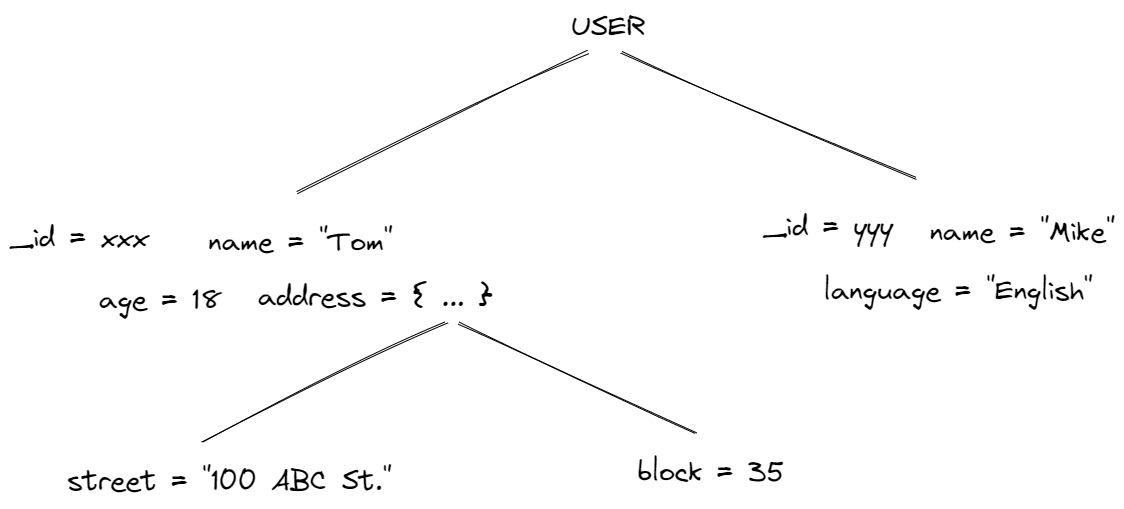
\includegraphics[width=250pt]{chapters/ch-database/figures/mongodb_tree.png}
	\caption{A demonstration of MongoDB storing data as object-of-object.} \label{ch:database:mongotree}
\end{figure}
In Fig. \ref{ch:database:mongotree}, the database is named ``USER''. The database contains two objects, also known as ``collections'' in MongoDB framework. Each collection has a few properties. Different collection may share common properties such as ``name'' in this example. Each of them can also have unique properties of its own such as ``age'', ``address'' and ``language'' in this example.

Different properties may have different types. For example, a property can be string, numeric, or an object, or a list of the above.

When querying MongoDB, the DBMS is able to return selected properties of documents that meet specific criteria, and order them in required order.

\vspace{0.1in}
\noindent \textbf{Installation}
\vspace{0.1in}

MongoDB, like many other DBMS, has both community and enterprise versions. MongoDB community server can be installed following the instructions in the official website
\begin{lstlisting}
https://www.mongodb.com/try/download/community
\end{lstlisting}
To interact with MongoDB DBMS, the quickest way is to use MongoDB shell (also known as ``mongosh''). A description of the shell can be found at
\begin{lstlisting}
https://www.mongodb.com/try/download/shell
\end{lstlisting}
Notice that when installing MongoDB server, it is possible that the server comes with MongoDB Compass, the GUI for MongoDB DBMS. The GUI can also be used to interact with the databases.

Different versions of MongoDB is provided. Choose the correct MongoDB version depending on the CPU and the OS of the machine. MongoDB community server installation size is about 500MB.

MongoDB provides enterprise service as part of its cloud solution, MongoDB Atlas, where user can deploy clusters to host databases. With proper gateway setup, the user can connect to MongoDB Atlas clusters from its local server to retrieve data or to manipulate the databases. MongoDB Atlas is not the covered in this notebook.

\vspace{0.1in}
\noindent \textbf{Basic Global Operations}
\vspace{0.1in}

After installing both MongoDB server and MonghDB shell, use \verb|mongosh| in the command line to login to the DBMS. JavaScript-like commands are used to manipulate the database, including creating databases and inserting data.

The object \verb|db| contains many methods using which the user can access and modify the basic configurations of the database. For example,
\begin{lstlisting}
> db.version()
\end{lstlisting}
gives the version of the database server. More commands can be found using \verb|db.help()|. Some commonly used commands are listed in Table \ref{ch:db:tab:mongodbbasics}.
\begin{table}
	\centering \caption{MongoDB basic commands.}\label{ch:db:tab:mongodbbasics}
	\begin{tabularx}{\textwidth}{lX}
		\hline
		Command & Description \\ \hline
        \verb|db.help()| & Show a list of methods of \verb|db| object. \\ \hdashline
		\verb|db.version()| & Show database server version. \\ \hdashline
        \verb|db.getUsers()| & Show users. \\ \hdashline
        \verb|db.createUser(<content>)| & Create a user. The username, password, roles, etc., needs to be included in the \verb|<content>| area. \\ \hdashline
        \verb|db.dropUser(<username>)| & Drop a user. \\ \hdashline
        \verb|db.dropDatabase()| & Drop current database. \\ \hdashline
		\verb|db.status()| & Show the basic status of the currently selected database, such as its name, number of collections, storage size, etc.  \\ \hdashline
        \verb|db.getUsers()| & Show users. \\
		 \hline
	\end{tabularx}
\end{table}

To display the existing databases, use
\begin{lstlisting}
> show dbs
\end{lstlisting}
On a clean installation, the above should return the 3 default databases, \verb|admin|, \verb|config| and \verb|local|. To change to a particular database, use
\begin{lstlisting}
> use <database_name>
\end{lstlisting}
Notice that there is no ``create database'' command in MongoDB. To create a database, switch to that database using the above command (even though it does not exist yet), and create some data such as a collection there. The database will be automatically created. This is again a feature closely related to JavaScript.

\vspace{0.1in}
\noindent \textbf{Data Format}
\vspace{0.1in}

MongoDB is a document-oriented database program. The data is stored in the format of ``binary JSON'' (BSON), which can be taken as an extension of JSON that supports more data types. Since BSON and JSON have a strong connection to the JavaScript object datatype, which looks very similar to a ``dictionary'', one may claim that MongoDB uses key-value pairs to store data. That statement is partially correct because BSON indeed adopts key-value pair structure to store data, but it may over simplifies the reality and might be misleading sometimes. In fact, BSON supports much more complicated data types other than string-to-string, such as array and nested objects.

JSON supports 6 datatypes: number, string, boolean (true or false), object, array and null. Notice that JSON is text-based, which is essentially a string. It is a notation of data. It does not concern how the data would be stored and used in the program who takes JSON as the input file. For example, from JSON's point of view, it does not distinguish different types of number, being integer or float or double. In JSON, it is just a notation of number, say ``$108$''. It is the program's responsibility to decide how to treat the number, either as an integer, or as a 32-bit float, or a 64-bit float.

BSON, on the other hand, is binary-based, which is essentially a list of binary numbers. This makes BSON more efficient (but less flexible and more difficult to use sometimes) than JSON. In BSON, more datatypes are supported, including: double (64-bit float), string, object, array, binary data (a binary string), object id, boolean, date, null, regular expression, JavaScript code, 32-bit integer, 64-bit integer, timestamp, etc. When using BSON, the user needs to be more specific on how the data should be stored. For example, for a number ``$108$'', the user needs to specify whether to store it as a 32-bit integer or a 64-bit integer, or maybe as a 64-bit float.

Both JSON and BSON are intuitive and human-readable. MongoDB uses BSON due to its enhanced capability.

\vspace{0.1in}
\noindent \textbf{Collection}
\vspace{0.1in}

A MongoDB database contains multiple collections. A collection is similar to a table in an RDB in the sense that it is the ``host'' of similar data. However, unlike tables where schematics such as column names and datatypes are enforced upon creation of the table, a collection does not enforce fields and data types. An example of creating a collection inside a database is given below.
\begin{lstlisting}
> use testdb
> db.createCollection("users")
\end{lstlisting}
Use \verb|show collections| to show the collections in the current database.

Data can be installed into a collection. An entry to be inserted to a collection, corresponding with a row of a table in RDB, is called a document. It is possible to insert one or multiple entries at a time. To insert documents, first prepare the document in BSON format. For example, consider the following documents.
\begin{lstlisting}
{
  name: "Alice",
  age: 20,
  address: "123 Center Park",
  hobbies: ["football", "reading"],
  parents: {
    father: "Chris",
    mother: "Kite"
  }
}

{
  name: "Bob",
  age: Long.fromNumber(25),
  address: "135 Center Park",
  hobbies: BSON.Array(["basketball", "jogging"])
}
\end{lstlisting}
Notice that user ``Alice'' and ``Bob'' are represented by JSON and BSON, respectively. MongoDB uses BSON internally, but it can also take JSON as input, in which case MongoDB driver converts JSON to BSON.

Then use the following syntax to insert the document into the collection.
\begin{lstlisting}
db.<collection_name>.insertOne({...})
db.<collection_name>.insertMany([{...}, {...}, {...}])
\end{lstlisting}
where \verb|{...}| is the document in JSON or BSON format as shown earlier. To make it more readable, consider do the following instead.
\begin{lstlisting}
const doc = {...};
db.<collection_name>.insertOne(doc)
\end{lstlisting}
which first store the document in \verb|doc|, then pass it to \verb|insertOne()| method. Upon successful insertion, an insert id (also known as object id) will be created automatically.




\vspace{0.1in}
\noindent \textbf{DBMS API}
\vspace{0.1in}




\subsection{Redis}





\subsection{AllegroGraph}





\section{Database Accessory}

\subsection{RDB Interface with Python}

Python provides variety of libraries to access RDS, many of which use embedded SQL codes to interact with the DBMS. Depending on the DBMS, different libraries and commands can be used, some of which more general and the other more specific to a particular DBMS.

In this section, both \verb|pandas| and \verb|mariadb| libraries are introduced. The \verb|pandas| library provides data manipulation and analysis tools, and it provides \verb|pandas.io.sql| that allows connecting to a DBMS and embedding SQL commands into the python code. The \verb|mariadb| library, on the other hand, is dedicated for MariaDB connection. Like \verb|pandas.io.sql|, it also allows embedding SQL commands to interface the DMBS.

As pre-requisitions, make sure that the following has been done.
\begin{itemize}
	\item The DBMS has been configured to allow remote access.
	\item Make sure that an account has been registered in DBMS that has the privilege of operation from a remote machine.
	\item Make sure that the firewall configuration is correct.
\end{itemize}

For DBMS configuration, in the case of MariaDB, use the following code in the shell to check the location of the configuration files.
\begin{lstlisting}
$ mysqld --help --verbose
\end{lstlisting}
Typical locations of the configuration files are \verb|/etc/my.cnf| and \verb|/etc/mysql/my.cnf|. In the configuration file, use the following to disable binding address.
\begin{lstlisting}
[mysqld]
skip-networking=0
skip-bind-address
\end{lstlisting}

For account setup, in the DBMS console, use something like
\begin{lstlisting}
> GRANT ALL PRIVILEGES ON *.* TO '<user-name>'@'<ip-address>' IDENTIFIED BY '<user-password>' WITH GRANT OPTION;
\end{lstlisting}
where \verb|'<ip-address>'| is the remote machine that runs the Python program. If the Python codes are running locally, simply use \verb|'localhost'|.

It might be necessary to install MariaDB database development files in the DMBS host machine for the Python libraries to be introduced to function properly. Install the development as follows.
\begin{lstlisting}
$ sudo apt install libmariadb-dev
\end{lstlisting}

\vspace{0.1in}
\noindent \textbf{PANDAS Library}
\vspace{0.1in}

Python library \verb|pandas| is one of the essential libraries for data analysis. It provides flexible interfaces and tools for data reading and processing and works very well with different data formats and engines including CSV, EXCEL and DBMS. This section focuses mainly on the interaction of \verb|pandas| with DBMS. Therefore, the detailed use of \verb|pandas| for data analysis, etc., are not covered in this section.

A class \verb|pandas.DataFrame| is defined in \verb|pandas| as the backbone to store and process data. The data attribute of \verb|pandas.DataFrame| is a \verb|numpy| array. Many functions are provided to read different data formats into \verb|pandas| data frame, which makes reading data easy and convenient. An example of reading a CSV file is given below.
\begin{lstlisting}
import pandas as pd
df = pd.read_csv(<file-name>)
print(df)
print(df.head(<number>))
print(df.tail(<number>))
print(df.info())
\end{lstlisting}
where \verb|head()|, \verb|tail()| gives the first and last rows of the data frame, and \verb|info()| checks the data frame basic information including shape and data types of the columns. Check \verb|df.columns| for all the columns of the data frame. Details specific to a column can be accessed via \verb|df.[<column-name>]|. Many functions are provided to further abstract the details, such as grouping and counting. Use \verb|df.loc(<row-index-list>, <column-name-list>)| to check the content of specified rows and columns.

With \verb|pandas| and other relavent libraries, Python can connect to a database and execute a query. An example of using \verb|pandas| to connect to an Microsoft SQL server and implement a query is given below. Notice that different DBMS may require different database connectivity driver standards, and there are mainly two of them, namely open database connectivity (ODBC) and Java database connectivity (JDBC). Microsoft adopts ODBC, and a separate package is required in the Python program to connect to the Microsoft SQL server.
\begin{lstlisting}
import pyodbc
import pandas.io.sql as psql

server = "<server-url>,<port>"
database = "<database>"
uid = "<uid>"
pwd = "<pwd>"
driver = "<driver>" # such as "{ODBC Driver 17 for SQL Server}"

# connect to database
conn = pyodbc.connect(
	server = server,
	database = database,
	uid = uid,
	pwd = pwd,
	driver = driver
)

# get cursor
cursor = conn.cursor()

# execute sql command
query = """<query>"""
runs = psql.read_sql_query(query, conn)
\end{lstlisting}
The above codes returns a data frame corresponding to the result set of the query string, which is saved in \verb|runs|.

\vspace{0.1in}
\noindent \textbf{MARIADB Library}
\vspace{0.1in}

Use the following code to test connectivity from Python to the database.
\begin{lstlisting}
import mariadb
import sys

user = "<user>"
password = "<password>"
host = "<server-url>"
port = "<port>" # MariaDB default: 3306
database = "<database>"

# connect to database
try:
	conn = mariadb.connect(
		user = user,
		password = password,
		host = host,
		port = port,
		database = database
	)
except mariadb.Error as e:
	print(f"Error connecting to MariaDB Platform: {e}")
	sys.exit(1)

# get cursor
cur = conn.cursor()

# execute sql command
cur.execute("<sql-command>")
\end{lstlisting}
Notice that for query, the result is stored in the cursor object. Use a for loop to view the results.
